\documentclass[1p]{elsarticle_modified}
%\bibliographystyle{elsarticle-num}

%\usepackage[colorlinks]{hyperref}
%\usepackage{abbrmath_seonhwa} %\Abb, \Ascr, \Acal ,\Abf, \Afrak
\usepackage{amsfonts}
\usepackage{amssymb}
\usepackage{amsmath}
\usepackage{amsthm}
\usepackage{scalefnt}
\usepackage{amsbsy}
\usepackage{kotex}
\usepackage{caption}
\usepackage{subfig}
\usepackage{color}
\usepackage{graphicx}
\usepackage{xcolor} %% white, black, red, green, blue, cyan, magenta, yellow
\usepackage{float}
\usepackage{setspace}
\usepackage{hyperref}

\usepackage{tikz}
\usetikzlibrary{arrows}

\usepackage{multirow}
\usepackage{array} % fixed length table
\usepackage{hhline}

%%%%%%%%%%%%%%%%%%%%%
\makeatletter
\renewcommand*\env@matrix[1][\arraystretch]{%
	\edef\arraystretch{#1}%
	\hskip -\arraycolsep
	\let\@ifnextchar\new@ifnextchar
	\array{*\c@MaxMatrixCols c}}
\makeatother %https://tex.stackexchange.com/questions/14071/how-can-i-increase-the-line-spacing-in-a-matrix
%%%%%%%%%%%%%%%

\usepackage[normalem]{ulem}

\newcommand{\msout}[1]{\ifmmode\text{\sout{\ensuremath{#1}}}\else\sout{#1}\fi}
%SOURCE: \msout is \stkout macro in https://tex.stackexchange.com/questions/20609/strikeout-in-math-mode

\newcommand{\cancel}[1]{
	\ifmmode
	{\color{red}\msout{#1}}
	\else
	{\color{red}\sout{#1}}
	\fi
}

\newcommand{\add}[1]{
	{\color{blue}\uwave{#1}}
}

\newcommand{\replace}[2]{
	\ifmmode
	{\color{red}\msout{#1}}{\color{blue}\uwave{#2}}
	\else
	{\color{red}\sout{#1}}{\color{blue}\uwave{#2}}
	\fi
}

\newcommand{\Sol}{\mathcal{S}} %segment
\newcommand{\D}{D} %diagram
\newcommand{\A}{\mathcal{A}} %arc


%%%%%%%%%%%%%%%%%%%%%%%%%%%%%5 test

\def\sl{\operatorname{\textup{SL}}(2,\Cbb)}
\def\psl{\operatorname{\textup{PSL}}(2,\Cbb)}
\def\quan{\mkern 1mu \triangleright \mkern 1mu}

\theoremstyle{definition}
\newtheorem{thm}{Theorem}[section]
\newtheorem{prop}[thm]{Proposition}
\newtheorem{lem}[thm]{Lemma}
\newtheorem{ques}[thm]{Question}
\newtheorem{cor}[thm]{Corollary}
\newtheorem{defn}[thm]{Definition}
\newtheorem{exam}[thm]{Example}
\newtheorem{rmk}[thm]{Remark}
\newtheorem{alg}[thm]{Algorithm}

\newcommand{\I}{\sqrt{-1}}
\begin{document}

%\begin{frontmatter}
%
%\title{Boundary parabolic representations of knots up to 8 crossings}
%
%%% Group authors per affiliation:
%\author{Yunhi Cho} 
%\address{Department of Mathematics, University of Seoul, Seoul, Korea}
%\ead{yhcho@uos.ac.kr}
%
%
%\author{Seonhwa Kim} %\fnref{s_kim}}
%\address{Center for Geometry and Physics, Institute for Basic Science, Pohang, 37673, Korea}
%\ead{ryeona17@ibs.re.kr}
%
%\author{Hyuk Kim}
%\address{Department of Mathematical Sciences, Seoul National University, Seoul 08826, Korea}
%\ead{hyukkim@snu.ac.kr}
%
%\author{Seokbeom Yoon}
%\address{Department of Mathematical Sciences, Seoul National University, Seoul, 08826,  Korea}
%\ead{sbyoon15@snu.ac.kr}
%
%\begin{abstract}
%We find all boundary parabolic representation of knots up to 8 crossings.
%
%\end{abstract}
%\begin{keyword}
%    \MSC[2010] 57M25 
%\end{keyword}
%
%\end{frontmatter}

%\linenumbers
%\tableofcontents
%
\newcommand\colored[1]{\textcolor{white}{\rule[-0.35ex]{0.8em}{1.4ex}}\kern-0.8em\color{red} #1}%
%\newcommand\colored[1]{\textcolor{white}{ #1}\kern-2.17ex	\textcolor{white}{ #1}\kern-1.81ex	\textcolor{white}{ #1}\kern-2.15ex\color{red}#1	}

{\Large $\underline{12n_{0621}~(K12n_{0621})}$}

\setlength{\tabcolsep}{10pt}
\renewcommand{\arraystretch}{1.6}
\vspace{1cm}\begin{tabular}{m{100pt}>{\centering\arraybackslash}m{274pt}}
\multirow{5}{120pt}{
	\centering
	\includegraphics[width=112pt]{../../../GIT/diagram.site/Diagrams/png/2710_12n_0621.png}\\
\ \ \ A knot diagram\footnotemark}&
\allowdisplaybreaks
\textbf{Linearized knot diagam} \\
\cline{2-2}
 &
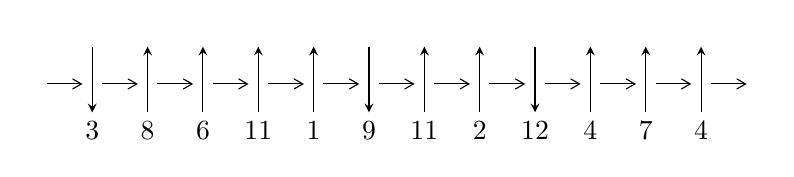
\begin{tikzpicture}[x=20pt, y=17pt]
	% nodes
	\node (C0) at (0, 0) {};
	\node (C1) at (1, 0) {};
	\node (C1U) at (1, +1) {};
	\node (C1D) at (1, -1) {3};

	\node (C2) at (2, 0) {};
	\node (C2U) at (2, +1) {};
	\node (C2D) at (2, -1) {8};

	\node (C3) at (3, 0) {};
	\node (C3U) at (3, +1) {};
	\node (C3D) at (3, -1) {6};

	\node (C4) at (4, 0) {};
	\node (C4U) at (4, +1) {};
	\node (C4D) at (4, -1) {11};

	\node (C5) at (5, 0) {};
	\node (C5U) at (5, +1) {};
	\node (C5D) at (5, -1) {1};

	\node (C6) at (6, 0) {};
	\node (C6U) at (6, +1) {};
	\node (C6D) at (6, -1) {9};

	\node (C7) at (7, 0) {};
	\node (C7U) at (7, +1) {};
	\node (C7D) at (7, -1) {11};

	\node (C8) at (8, 0) {};
	\node (C8U) at (8, +1) {};
	\node (C8D) at (8, -1) {2};

	\node (C9) at (9, 0) {};
	\node (C9U) at (9, +1) {};
	\node (C9D) at (9, -1) {12};

	\node (C10) at (10, 0) {};
	\node (C10U) at (10, +1) {};
	\node (C10D) at (10, -1) {4};

	\node (C11) at (11, 0) {};
	\node (C11U) at (11, +1) {};
	\node (C11D) at (11, -1) {7};

	\node (C12) at (12, 0) {};
	\node (C12U) at (12, +1) {};
	\node (C12D) at (12, -1) {4};
	\node (C13) at (13, 0) {};

	% arrows
	\draw[->,>={angle 60}]
	(C0) edge (C1) (C1) edge (C2) (C2) edge (C3) (C3) edge (C4) (C4) edge (C5) (C5) edge (C6) (C6) edge (C7) (C7) edge (C8) (C8) edge (C9) (C9) edge (C10) (C10) edge (C11) (C11) edge (C12) (C12) edge (C13) ;	\draw[->,>=stealth]
	(C1U) edge (C1D) (C2D) edge (C2U) (C3D) edge (C3U) (C4D) edge (C4U) (C5D) edge (C5U) (C6U) edge (C6D) (C7D) edge (C7U) (C8D) edge (C8U) (C9U) edge (C9D) (C10D) edge (C10U) (C11D) edge (C11U) (C12D) edge (C12U) ;
	\end{tikzpicture} \\
\hhline{~~} \\& 
\textbf{Solving Sequence} \\ \cline{2-2} 
 &
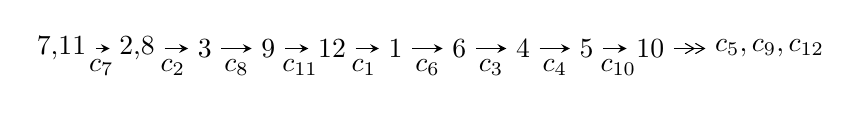
\begin{tikzpicture}[x=23pt, y=7pt]
	% node
	\node (A0) at (-1/8, 0) {7,11};
	\node (A1) at (17/16, 0) {2,8};
	\node (A2) at (17/8, 0) {3};
	\node (A3) at (25/8, 0) {9};
	\node (A4) at (33/8, 0) {12};
	\node (A5) at (41/8, 0) {1};
	\node (A6) at (49/8, 0) {6};
	\node (A7) at (57/8, 0) {4};
	\node (A8) at (65/8, 0) {5};
	\node (A9) at (73/8, 0) {10};
	\node (C1) at (1/2, -1) {$c_{7}$};
	\node (C2) at (13/8, -1) {$c_{2}$};
	\node (C3) at (21/8, -1) {$c_{8}$};
	\node (C4) at (29/8, -1) {$c_{11}$};
	\node (C5) at (37/8, -1) {$c_{1}$};
	\node (C6) at (45/8, -1) {$c_{6}$};
	\node (C7) at (53/8, -1) {$c_{3}$};
	\node (C8) at (61/8, -1) {$c_{4}$};
	\node (C9) at (69/8, -1) {$c_{10}$};
	\node (A10) at (11, 0) {$c_{5},c_{9},c_{12}$};

	% edge
	\draw[->,>=stealth]	
	(A0) edge (A1) (A1) edge (A2) (A2) edge (A3) (A3) edge (A4) (A4) edge (A5) (A5) edge (A6) (A6) edge (A7) (A7) edge (A8) (A8) edge (A9) ;
	\draw[->>,>={angle 60}]	
	(A9) edge (A10);
\end{tikzpicture} \\ 

\end{tabular} \\

\footnotetext{
The image of knot diagram is generated by the software ``\textbf{Draw programme}" developed by Andrew Bartholomew(\url{http://www.layer8.co.uk/maths/draw/index.htm\#Running-draw}), where we modified some parts for our purpose(\url{https://github.com/CATsTAILs/LinksPainter}).
}\phantom \\ \newline 
\centering \textbf{Ideals for irreducible components\footnotemark of $X_{\text{par}}$} 
 
\begin{align*}
I^u_{1}&=\langle 
-2.93614\times10^{247} u^{74}-5.74396\times10^{247} u^{73}+\cdots+4.12848\times10^{248} b-5.70956\times10^{248},\\
\phantom{I^u_{1}}&\phantom{= \langle  }1.02425\times10^{248} u^{74}+2.08487\times10^{248} u^{73}+\cdots+8.25697\times10^{248} a+4.56133\times10^{249},\;u^{75}+2 u^{74}+\cdots+14 u+1\rangle \\
I^u_{2}&=\langle 
-3110107574105 u^{27}+3424303947942 u^{26}+\cdots+1161098476808 b-3547833988250,\\
\phantom{I^u_{2}}&\phantom{= \langle  }8831335807959 u^{27}-8605065406950 u^{26}+\cdots+1161098476808 a+15780292874526,\\
\phantom{I^u_{2}}&\phantom{= \langle  }u^{28}- u^{27}+\cdots+2 u+1\rangle \\
\\
\end{align*}
\raggedright * 2 irreducible components of $\dim_{\mathbb{C}}=0$, with total 103 representations.\\
\footnotetext{All coefficients of polynomials are rational numbers. But the coefficients are sometimes approximated in decimal forms when there is not enough margin.}
\newpage
\renewcommand{\arraystretch}{1}
\centering \section*{I. $I^u_{1}= \langle -2.94\times10^{247} u^{74}-5.74\times10^{247} u^{73}+\cdots+4.13\times10^{248} b-5.71\times10^{248},\;1.02\times10^{248} u^{74}+2.08\times10^{248} u^{73}+\cdots+8.26\times10^{248} a+4.56\times10^{249},\;u^{75}+2 u^{74}+\cdots+14 u+1 \rangle$}
\flushleft \textbf{(i) Arc colorings}\\
\begin{tabular}{m{7pt} m{180pt} m{7pt} m{180pt} }
\flushright $a_{7}=$&$\begin{pmatrix}1\\0\end{pmatrix}$ \\
\flushright $a_{11}=$&$\begin{pmatrix}0\\u\end{pmatrix}$ \\
\flushright $a_{2}=$&$\begin{pmatrix}-0.124047 u^{74}-0.252498 u^{73}+\cdots-19.1786 u-5.52422\\0.0711190 u^{74}+0.139130 u^{73}+\cdots+10.8001 u+1.38297\end{pmatrix}$ \\
\flushright $a_{8}=$&$\begin{pmatrix}1\\- u^2\end{pmatrix}$ \\
\flushright $a_{3}=$&$\begin{pmatrix}-0.0562848 u^{74}-0.118506 u^{73}+\cdots-8.19273 u-4.13684\\0.0684905 u^{74}+0.133802 u^{73}+\cdots+10.8464 u+1.38143\end{pmatrix}$ \\
\flushright $a_{9}=$&$\begin{pmatrix}0.438977 u^{74}+0.862197 u^{73}+\cdots+60.1161 u+7.08484\\-0.0864639 u^{74}-0.173895 u^{73}+\cdots-16.5768 u-0.680945\end{pmatrix}$ \\
\flushright $a_{12}=$&$\begin{pmatrix}u\\u\end{pmatrix}$ \\
\flushright $a_{1}=$&$\begin{pmatrix}-0.525441 u^{74}-1.03609 u^{73}+\cdots-76.6929 u-7.76579\\0.0786284 u^{74}+0.164196 u^{73}+\cdots+22.0608 u+0.532563\end{pmatrix}$ \\
\flushright $a_{6}=$&$\begin{pmatrix}0.0636480 u^{74}+0.130102 u^{73}+\cdots+42.4904 u-4.45507\\0.0800330 u^{74}+0.158503 u^{73}+\cdots+4.65689 u+2.07918\end{pmatrix}$ \\
\flushright $a_{4}=$&$\begin{pmatrix}0.456997 u^{74}+0.856393 u^{73}+\cdots-37.0559 u+4.65699\\-0.0506077 u^{74}-0.0881954 u^{73}+\cdots+4.56215 u-0.218959\end{pmatrix}$ \\
\flushright $a_{5}=$&$\begin{pmatrix}0.456997 u^{74}+0.856393 u^{73}+\cdots-37.0559 u+4.65699\\-0.0587013 u^{74}-0.106320 u^{73}+\cdots+4.21274 u-0.276560\end{pmatrix}$ \\
\flushright $a_{10}=$&$\begin{pmatrix}0.436497 u^{74}+0.856775 u^{73}+\cdots+59.7977 u+7.09963\\-0.0889433 u^{74}-0.179317 u^{73}+\cdots-16.8952 u-0.666156\end{pmatrix}$\\&\end{tabular}
\flushleft \textbf{(ii) Obstruction class $= -1$}\\~\\
\flushleft \textbf{(iii) Cusp Shapes $= -0.296278 u^{74}-0.494942 u^{73}+\cdots+11.7325 u+14.5179$}\\~\\
\newpage\renewcommand{\arraystretch}{1}
\flushleft \textbf{(iv) u-Polynomials at the component}\newline \\
\begin{tabular}{m{50pt}|m{274pt}}
Crossings & \hspace{64pt}u-Polynomials at each crossing \\
\hline $$\begin{aligned}c_{1}\end{aligned}$$&$\begin{aligned}
&u^{75}+37 u^{74}+\cdots-48 u-16
\end{aligned}$\\
\hline $$\begin{aligned}c_{2},c_{8}\end{aligned}$$&$\begin{aligned}
&u^{75}+u^{74}+\cdots-8 u-4
\end{aligned}$\\
\hline $$\begin{aligned}c_{3}\end{aligned}$$&$\begin{aligned}
&u^{75}+9 u^{74}+\cdots-284 u-19
\end{aligned}$\\
\hline $$\begin{aligned}c_{4},c_{10}\end{aligned}$$&$\begin{aligned}
&u^{75}- u^{74}+\cdots-2058072 u-145372
\end{aligned}$\\
\hline $$\begin{aligned}c_{5}\end{aligned}$$&$\begin{aligned}
&u^{75}-3 u^{74}+\cdots+2493542 u-4382428
\end{aligned}$\\
\hline $$\begin{aligned}c_{6}\end{aligned}$$&$\begin{aligned}
&u^{75}-5 u^{74}+\cdots+54618 u-5068
\end{aligned}$\\
\hline $$\begin{aligned}c_{7},c_{11}\end{aligned}$$&$\begin{aligned}
&u^{75}-2 u^{74}+\cdots+14 u-1
\end{aligned}$\\
\hline $$\begin{aligned}c_{9}\end{aligned}$$&$\begin{aligned}
&u^{75}-7 u^{74}+\cdots+1121 u-691
\end{aligned}$\\
\hline $$\begin{aligned}c_{12}\end{aligned}$$&$\begin{aligned}
&u^{75}+3 u^{74}+\cdots-60886 u-6196
\end{aligned}$\\
\hline
\end{tabular}\\~\\
\newpage\renewcommand{\arraystretch}{1}
\flushleft \textbf{(v) Riley Polynomials at the component}\newline \\
\begin{tabular}{m{50pt}|m{274pt}}
Crossings & \hspace{64pt}Riley Polynomials at each crossing \\
\hline $$\begin{aligned}c_{1}\end{aligned}$$&$\begin{aligned}
&y^{75}+21 y^{74}+\cdots+1408 y-256
\end{aligned}$\\
\hline $$\begin{aligned}c_{2},c_{8}\end{aligned}$$&$\begin{aligned}
&y^{75}+37 y^{74}+\cdots-48 y-16
\end{aligned}$\\
\hline $$\begin{aligned}c_{3}\end{aligned}$$&$\begin{aligned}
&y^{75}- y^{74}+\cdots-9366 y-361
\end{aligned}$\\
\hline $$\begin{aligned}c_{4},c_{10}\end{aligned}$$&$\begin{aligned}
&y^{75}+103 y^{74}+\cdots-180569463856 y-21133018384
\end{aligned}$\\
\hline $$\begin{aligned}c_{5}\end{aligned}$$&$\begin{aligned}
&y^{75}+59 y^{74}+\cdots+152134872802076 y-19205675175184
\end{aligned}$\\
\hline $$\begin{aligned}c_{6}\end{aligned}$$&$\begin{aligned}
&y^{75}-19 y^{74}+\cdots+614373132 y-25684624
\end{aligned}$\\
\hline $$\begin{aligned}c_{7},c_{11}\end{aligned}$$&$\begin{aligned}
&y^{75}+56 y^{74}+\cdots-26 y-1
\end{aligned}$\\
\hline $$\begin{aligned}c_{9}\end{aligned}$$&$\begin{aligned}
&y^{75}-111 y^{74}+\cdots+20483025 y-477481
\end{aligned}$\\
\hline $$\begin{aligned}c_{12}\end{aligned}$$&$\begin{aligned}
&y^{75}+105 y^{74}+\cdots+337608668 y-38390416
\end{aligned}$\\
\hline
\end{tabular}\\~\\
\newpage\flushleft \textbf{(vi) Complex Volumes and Cusp Shapes}
$$\begin{array}{c|c|c}  
\text{Solutions to }I^u_{1}& \I (\text{vol} + \sqrt{-1}CS) & \text{Cusp shape}\\
 \hline 
\begin{aligned}
u &= -0.338490 + 1.014360 I \\
a &= -0.083989 + 0.737529 I \\
b &= -0.225489 + 0.455556 I\end{aligned}
 & -1.59254 - 2.41045 I & \phantom{-0.000000 } 0 \\ \hline\begin{aligned}
u &= -0.338490 - 1.014360 I \\
a &= -0.083989 - 0.737529 I \\
b &= -0.225489 - 0.455556 I\end{aligned}
 & -1.59254 + 2.41045 I & \phantom{-0.000000 } 0 \\ \hline\begin{aligned}
u &= \phantom{-}0.343964 + 0.853499 I \\
a &= -1.63427 + 3.28949 I \\
b &= \phantom{-}1.11108 + 2.10173 I\end{aligned}
 & -5.77417 + 1.98856 I & \phantom{-0.000000 } 0 \\ \hline\begin{aligned}
u &= \phantom{-}0.343964 - 0.853499 I \\
a &= -1.63427 - 3.28949 I \\
b &= \phantom{-}1.11108 - 2.10173 I\end{aligned}
 & -5.77417 - 1.98856 I & \phantom{-0.000000 } 0 \\ \hline\begin{aligned}
u &= \phantom{-}0.812407 + 0.295359 I \\
a &= -0.650857 - 0.548434 I \\
b &= -0.49354 + 1.63137 I\end{aligned}
 & \phantom{-}0.50070 - 3.88299 I & \phantom{-0.000000 } 0 \\ \hline\begin{aligned}
u &= \phantom{-}0.812407 - 0.295359 I \\
a &= -0.650857 + 0.548434 I \\
b &= -0.49354 - 1.63137 I\end{aligned}
 & \phantom{-}0.50070 + 3.88299 I & \phantom{-0.000000 } 0 \\ \hline\begin{aligned}
u &= \phantom{-}0.211341 + 1.118520 I \\
a &= -0.33364 + 1.80730 I \\
b &= \phantom{-}0.87362 + 1.28162 I\end{aligned}
 & -4.06339 - 1.03839 I & \phantom{-0.000000 } 0 \\ \hline\begin{aligned}
u &= \phantom{-}0.211341 - 1.118520 I \\
a &= -0.33364 - 1.80730 I \\
b &= \phantom{-}0.87362 - 1.28162 I\end{aligned}
 & -4.06339 + 1.03839 I & \phantom{-0.000000 } 0 \\ \hline\begin{aligned}
u &= -0.688873 + 0.501015 I \\
a &= -0.700829 - 0.337773 I \\
b &= -0.285517 + 0.188871 I\end{aligned}
 & \phantom{-}1.72423 - 1.07048 I & \phantom{-0.000000 } 0 \\ \hline\begin{aligned}
u &= -0.688873 - 0.501015 I \\
a &= -0.700829 + 0.337773 I \\
b &= -0.285517 - 0.188871 I\end{aligned}
 & \phantom{-}1.72423 + 1.07048 I & \phantom{-0.000000 } 0\\
 \hline 
 \end{array}$$\newpage$$\begin{array}{c|c|c}  
\text{Solutions to }I^u_{1}& \I (\text{vol} + \sqrt{-1}CS) & \text{Cusp shape}\\
 \hline 
\begin{aligned}
u &= \phantom{-}0.533903 + 1.016930 I \\
a &= \phantom{-}1.58173 - 1.65823 I \\
b &= -0.15810 - 1.89823 I\end{aligned}
 & -3.86944 + 5.81407 I & \phantom{-0.000000 } 0 \\ \hline\begin{aligned}
u &= \phantom{-}0.533903 - 1.016930 I \\
a &= \phantom{-}1.58173 + 1.65823 I \\
b &= -0.15810 + 1.89823 I\end{aligned}
 & -3.86944 - 5.81407 I & \phantom{-0.000000 } 0 \\ \hline\begin{aligned}
u &= -0.545651 + 1.035230 I \\
a &= -0.426292 + 0.404260 I \\
b &= \phantom{-}0.052141 + 0.213347 I\end{aligned}
 & \phantom{-}0.10985 - 3.67304 I & \phantom{-0.000000 } 0 \\ \hline\begin{aligned}
u &= -0.545651 - 1.035230 I \\
a &= -0.426292 - 0.404260 I \\
b &= \phantom{-}0.052141 - 0.213347 I\end{aligned}
 & \phantom{-}0.10985 + 3.67304 I & \phantom{-0.000000 } 0 \\ \hline\begin{aligned}
u &= -0.248881 + 0.790036 I \\
a &= -0.094181 + 1.033320 I \\
b &= -0.328403 + 1.126780 I\end{aligned}
 & -1.88152 - 2.41983 I & \phantom{-0.000000 } 0 \\ \hline\begin{aligned}
u &= -0.248881 - 0.790036 I \\
a &= -0.094181 - 1.033320 I \\
b &= -0.328403 - 1.126780 I\end{aligned}
 & -1.88152 + 2.41983 I & \phantom{-0.000000 } 0 \\ \hline\begin{aligned}
u &= \phantom{-}0.097339 + 1.218700 I \\
a &= \phantom{-}0.222120 - 0.272580 I \\
b &= -0.662838 - 0.164392 I\end{aligned}
 & -0.26158 + 2.14205 I & \phantom{-0.000000 } 0 \\ \hline\begin{aligned}
u &= \phantom{-}0.097339 - 1.218700 I \\
a &= \phantom{-}0.222120 + 0.272580 I \\
b &= -0.662838 + 0.164392 I\end{aligned}
 & -0.26158 - 2.14205 I & \phantom{-0.000000 } 0 \\ \hline\begin{aligned}
u &= \phantom{-}1.260860 + 0.012988 I \\
a &= -0.813627 + 0.273446 I \\
b &= \phantom{-}0.635193 - 0.683649 I\end{aligned}
 & -4.57011 - 3.93986 I & \phantom{-0.000000 } 0 \\ \hline\begin{aligned}
u &= \phantom{-}1.260860 - 0.012988 I \\
a &= -0.813627 - 0.273446 I \\
b &= \phantom{-}0.635193 + 0.683649 I\end{aligned}
 & -4.57011 + 3.93986 I & \phantom{-0.000000 } 0\\
 \hline 
 \end{array}$$\newpage$$\begin{array}{c|c|c}  
\text{Solutions to }I^u_{1}& \I (\text{vol} + \sqrt{-1}CS) & \text{Cusp shape}\\
 \hline 
\begin{aligned}
u &= \phantom{-}0.096237 + 1.263760 I \\
a &= \phantom{-}0.068326 + 0.488408 I \\
b &= -0.901195 - 0.026334 I\end{aligned}
 & -6.63701 + 4.14284 I & \phantom{-0.000000 } 0 \\ \hline\begin{aligned}
u &= \phantom{-}0.096237 - 1.263760 I \\
a &= \phantom{-}0.068326 - 0.488408 I \\
b &= -0.901195 + 0.026334 I\end{aligned}
 & -6.63701 - 4.14284 I & \phantom{-0.000000 } 0 \\ \hline\begin{aligned}
u &= -0.244538 + 1.249340 I \\
a &= \phantom{-}0.273380 + 0.486740 I \\
b &= -0.322007 + 0.572207 I\end{aligned}
 & -1.46648 - 2.68040 I & \phantom{-0.000000 } 0 \\ \hline\begin{aligned}
u &= -0.244538 - 1.249340 I \\
a &= \phantom{-}0.273380 - 0.486740 I \\
b &= -0.322007 - 0.572207 I\end{aligned}
 & -1.46648 + 2.68040 I & \phantom{-0.000000 } 0 \\ \hline\begin{aligned}
u &= \phantom{-}0.149500 + 1.265560 I \\
a &= -0.23660 + 1.50686 I \\
b &= -0.688027 + 1.076700 I\end{aligned}
 & -8.24845 + 3.84574 I & \phantom{-0.000000 } 0 \\ \hline\begin{aligned}
u &= \phantom{-}0.149500 - 1.265560 I \\
a &= -0.23660 - 1.50686 I \\
b &= -0.688027 - 1.076700 I\end{aligned}
 & -8.24845 - 3.84574 I & \phantom{-0.000000 } 0 \\ \hline\begin{aligned}
u &= \phantom{-}0.568915 + 1.158220 I \\
a &= \phantom{-}1.14020 - 1.97951 I \\
b &= -0.84223 - 2.39603 I\end{aligned}
 & -2.08797 + 9.01604 I & \phantom{-0.000000 } 0 \\ \hline\begin{aligned}
u &= \phantom{-}0.568915 - 1.158220 I \\
a &= \phantom{-}1.14020 + 1.97951 I \\
b &= -0.84223 + 2.39603 I\end{aligned}
 & -2.08797 - 9.01604 I & \phantom{-0.000000 } 0 \\ \hline\begin{aligned}
u &= \phantom{-}0.105585 + 1.294190 I \\
a &= -0.094589 - 0.455966 I \\
b &= -1.00362 - 1.24602 I\end{aligned}
 & -8.16649 + 0.01465 I & \phantom{-0.000000 } 0 \\ \hline\begin{aligned}
u &= \phantom{-}0.105585 - 1.294190 I \\
a &= -0.094589 + 0.455966 I \\
b &= -1.00362 + 1.24602 I\end{aligned}
 & -8.16649 - 0.01465 I & \phantom{-0.000000 } 0\\
 \hline 
 \end{array}$$\newpage$$\begin{array}{c|c|c}  
\text{Solutions to }I^u_{1}& \I (\text{vol} + \sqrt{-1}CS) & \text{Cusp shape}\\
 \hline 
\begin{aligned}
u &= \phantom{-}0.083185 + 1.303140 I \\
a &= -1.44819 + 1.43760 I \\
b &= -2.73221 + 1.68154 I\end{aligned}
 & -9.82572 + 5.04338 I & \phantom{-0.000000 } 0 \\ \hline\begin{aligned}
u &= \phantom{-}0.083185 - 1.303140 I \\
a &= -1.44819 - 1.43760 I \\
b &= -2.73221 - 1.68154 I\end{aligned}
 & -9.82572 - 5.04338 I & \phantom{-0.000000 } 0 \\ \hline\begin{aligned}
u &= \phantom{-}0.372696 + 1.256320 I \\
a &= -0.65580 + 1.84410 I \\
b &= \phantom{-}0.68355 + 2.03412 I\end{aligned}
 & -5.97939 + 1.25175 I & \phantom{-0.000000 } 0 \\ \hline\begin{aligned}
u &= \phantom{-}0.372696 - 1.256320 I \\
a &= -0.65580 - 1.84410 I \\
b &= \phantom{-}0.68355 - 2.03412 I\end{aligned}
 & -5.97939 - 1.25175 I & \phantom{-0.000000 } 0 \\ \hline\begin{aligned}
u &= \phantom{-}1.333380 + 0.173682 I \\
a &= \phantom{-}0.811498 - 0.849545 I \\
b &= -1.37253 + 1.88759 I\end{aligned}
 & \phantom{-}4.21365 + 1.49945 I & \phantom{-0.000000 } 0 \\ \hline\begin{aligned}
u &= \phantom{-}1.333380 - 0.173682 I \\
a &= \phantom{-}0.811498 + 0.849545 I \\
b &= -1.37253 - 1.88759 I\end{aligned}
 & \phantom{-}4.21365 - 1.49945 I & \phantom{-0.000000 } 0 \\ \hline\begin{aligned}
u &= -0.289653 + 1.324520 I \\
a &= -1.04672 - 1.72698 I \\
b &= -0.82792 - 2.61892 I\end{aligned}
 & -4.21139 - 0.24470 I & \phantom{-0.000000 } 0 \\ \hline\begin{aligned}
u &= -0.289653 - 1.324520 I \\
a &= -1.04672 + 1.72698 I \\
b &= -0.82792 + 2.61892 I\end{aligned}
 & -4.21139 + 0.24470 I & \phantom{-0.000000 } 0 \\ \hline\begin{aligned}
u &= -1.42651 + 0.03741 I \\
a &= \phantom{-}0.570335 + 0.464102 I \\
b &= -0.76187 - 1.78511 I\end{aligned}
 & \phantom{-}3.79263 - 2.20139 I & \phantom{-0.000000 } 0 \\ \hline\begin{aligned}
u &= -1.42651 - 0.03741 I \\
a &= \phantom{-}0.570335 - 0.464102 I \\
b &= -0.76187 + 1.78511 I\end{aligned}
 & \phantom{-}3.79263 + 2.20139 I & \phantom{-0.000000 } 0\\
 \hline 
 \end{array}$$\newpage$$\begin{array}{c|c|c}  
\text{Solutions to }I^u_{1}& \I (\text{vol} + \sqrt{-1}CS) & \text{Cusp shape}\\
 \hline 
\begin{aligned}
u &= \phantom{-}0.374818 + 0.350718 I \\
a &= -2.80026 + 0.39715 I \\
b &= \phantom{-}0.746495 + 0.170227 I\end{aligned}
 & -3.55538 - 2.70832 I & \phantom{-}5.95415 + 0.21604 I \\ \hline\begin{aligned}
u &= \phantom{-}0.374818 - 0.350718 I \\
a &= -2.80026 - 0.39715 I \\
b &= \phantom{-}0.746495 - 0.170227 I\end{aligned}
 & -3.55538 + 2.70832 I & \phantom{-}5.95415 - 0.21604 I \\ \hline\begin{aligned}
u &= \phantom{-}0.456613 + 0.215336 I \\
a &= -0.763234 - 0.254726 I \\
b &= -0.097092 + 1.163740 I\end{aligned}
 & -2.17924 - 1.79406 I & \phantom{-}3.71045 + 3.85861 I \\ \hline\begin{aligned}
u &= \phantom{-}0.456613 - 0.215336 I \\
a &= -0.763234 + 0.254726 I \\
b &= -0.097092 - 1.163740 I\end{aligned}
 & -2.17924 + 1.79406 I & \phantom{-}3.71045 - 3.85861 I \\ \hline\begin{aligned}
u &= -0.21547 + 1.48414 I \\
a &= -0.38029 - 1.54285 I \\
b &= -0.42424 - 2.38866 I\end{aligned}
 & -2.97425 - 7.62553 I & \phantom{-0.000000 } 0 \\ \hline\begin{aligned}
u &= -0.21547 - 1.48414 I \\
a &= -0.38029 + 1.54285 I \\
b &= -0.42424 + 2.38866 I\end{aligned}
 & -2.97425 + 7.62553 I & \phantom{-0.000000 } 0 \\ \hline\begin{aligned}
u &= \phantom{-}0.084889 + 0.487616 I \\
a &= -4.49287 - 0.57716 I \\
b &= -0.733448 - 0.772570 I\end{aligned}
 & -6.72101 - 4.29646 I & -3.76910 + 2.69049 I \\ \hline\begin{aligned}
u &= \phantom{-}0.084889 - 0.487616 I \\
a &= -4.49287 + 0.57716 I \\
b &= -0.733448 + 0.772570 I\end{aligned}
 & -6.72101 + 4.29646 I & -3.76910 - 2.69049 I \\ \hline\begin{aligned}
u &= -1.40921 + 0.57774 I \\
a &= -0.451526 + 0.502532 I \\
b &= -0.41328 - 2.67844 I\end{aligned}
 & -8.29796 - 0.94595 I & \phantom{-0.000000 } 0 \\ \hline\begin{aligned}
u &= -1.40921 - 0.57774 I \\
a &= -0.451526 - 0.502532 I \\
b &= -0.41328 + 2.67844 I\end{aligned}
 & -8.29796 + 0.94595 I & \phantom{-0.000000 } 0\\
 \hline 
 \end{array}$$\newpage$$\begin{array}{c|c|c}  
\text{Solutions to }I^u_{1}& \I (\text{vol} + \sqrt{-1}CS) & \text{Cusp shape}\\
 \hline 
\begin{aligned}
u &= \phantom{-}0.57774 + 1.46690 I \\
a &= -0.136989 - 0.135245 I \\
b &= \phantom{-}0.523608 - 0.380389 I\end{aligned}
 & -9.27086 + 10.48060 I & \phantom{-0.000000 } 0 \\ \hline\begin{aligned}
u &= \phantom{-}0.57774 - 1.46690 I \\
a &= -0.136989 + 0.135245 I \\
b &= \phantom{-}0.523608 + 0.380389 I\end{aligned}
 & -9.27086 - 10.48060 I & \phantom{-0.000000 } 0 \\ \hline\begin{aligned}
u &= \phantom{-}0.275445 + 0.320660 I \\
a &= -2.91158 - 0.02172 I \\
b &= \phantom{-}0.501597 - 0.568378 I\end{aligned}
 & -5.04243 - 2.17825 I & \phantom{-}3.70428 + 5.60941 I \\ \hline\begin{aligned}
u &= \phantom{-}0.275445 - 0.320660 I \\
a &= -2.91158 + 0.02172 I \\
b &= \phantom{-}0.501597 + 0.568378 I\end{aligned}
 & -5.04243 + 2.17825 I & \phantom{-}3.70428 - 5.60941 I \\ \hline\begin{aligned}
u &= \phantom{-}0.16408 + 1.56901 I \\
a &= -0.28564 + 1.78527 I \\
b &= -0.26882 + 3.41347 I\end{aligned}
 & -3.58764 + 6.75970 I & \phantom{-0.000000 } 0 \\ \hline\begin{aligned}
u &= \phantom{-}0.16408 - 1.56901 I \\
a &= -0.28564 - 1.78527 I \\
b &= -0.26882 - 3.41347 I\end{aligned}
 & -3.58764 - 6.75970 I & \phantom{-0.000000 } 0 \\ \hline\begin{aligned}
u &= \phantom{-}0.63107 + 1.45962 I \\
a &= \phantom{-}0.238033 - 0.112386 I \\
b &= \phantom{-}0.982552 - 0.988516 I\end{aligned}
 & -9.04107 + 2.56417 I & \phantom{-0.000000 } 0 \\ \hline\begin{aligned}
u &= \phantom{-}0.63107 - 1.45962 I \\
a &= \phantom{-}0.238033 + 0.112386 I \\
b &= \phantom{-}0.982552 + 0.988516 I\end{aligned}
 & -9.04107 - 2.56417 I & \phantom{-0.000000 } 0 \\ \hline\begin{aligned}
u &= \phantom{-}0.04084 + 1.60964 I \\
a &= \phantom{-}0.75777 - 1.77433 I \\
b &= \phantom{-}1.43111 - 3.73653 I\end{aligned}
 & -12.12460 - 1.13507 I & \phantom{-0.000000 } 0 \\ \hline\begin{aligned}
u &= \phantom{-}0.04084 - 1.60964 I \\
a &= \phantom{-}0.75777 + 1.77433 I \\
b &= \phantom{-}1.43111 + 3.73653 I\end{aligned}
 & -12.12460 + 1.13507 I & \phantom{-0.000000 } 0\\
 \hline 
 \end{array}$$\newpage$$\begin{array}{c|c|c}  
\text{Solutions to }I^u_{1}& \I (\text{vol} + \sqrt{-1}CS) & \text{Cusp shape}\\
 \hline 
\begin{aligned}
u &= -0.34679 + 1.57824 I \\
a &= -0.09367 - 1.58863 I \\
b &= \phantom{-}1.63442 - 2.48460 I\end{aligned}
 & -15.6106 - 6.7181 I & \phantom{-0.000000 } 0 \\ \hline\begin{aligned}
u &= -0.34679 - 1.57824 I \\
a &= -0.09367 + 1.58863 I \\
b &= \phantom{-}1.63442 + 2.48460 I\end{aligned}
 & -15.6106 + 6.7181 I & \phantom{-0.000000 } 0 \\ \hline\begin{aligned}
u &= -1.63199 + 0.04625 I \\
a &= -0.551410 + 0.644182 I \\
b &= \phantom{-}0.84326 - 2.91872 I\end{aligned}
 & -6.99114 + 8.56653 I & \phantom{-0.000000 } 0 \\ \hline\begin{aligned}
u &= -1.63199 - 0.04625 I \\
a &= -0.551410 - 0.644182 I \\
b &= \phantom{-}0.84326 + 2.91872 I\end{aligned}
 & -6.99114 - 8.56653 I & \phantom{-0.000000 } 0 \\ \hline\begin{aligned}
u &= -0.68541 + 1.54649 I \\
a &= \phantom{-}0.83167 + 1.45807 I \\
b &= -0.83970 + 3.36363 I\end{aligned}
 & -11.8545 - 16.4570 I & \phantom{-0.000000 } 0 \\ \hline\begin{aligned}
u &= -0.68541 - 1.54649 I \\
a &= \phantom{-}0.83167 - 1.45807 I \\
b &= -0.83970 - 3.36363 I\end{aligned}
 & -11.8545 + 16.4570 I & \phantom{-0.000000 } 0 \\ \hline\begin{aligned}
u &= -0.289488\phantom{ +0.000000I} \\
a &= -0.732575\phantom{ +0.000000I} \\
b &= -0.350214\phantom{ +0.000000I}\end{aligned}
 & \phantom{-}0.735693\phantom{ +0.000000I} & \phantom{-}13.9000\phantom{ +0.000000I} \\ \hline\begin{aligned}
u &= -0.87530 + 1.54498 I \\
a &= \phantom{-}0.88420 + 1.17471 I \\
b &= -1.16957 + 3.16272 I\end{aligned}
 & -11.35710 - 7.66415 I & \phantom{-0.000000 } 0 \\ \hline\begin{aligned}
u &= -0.87530 - 1.54498 I \\
a &= \phantom{-}0.88420 - 1.17471 I \\
b &= -1.16957 - 3.16272 I\end{aligned}
 & -11.35710 + 7.66415 I & \phantom{-0.000000 } 0 \\ \hline\begin{aligned}
u &= \phantom{-}0.0114997 + 0.0911495 I \\
a &= -3.59923 - 1.96297 I \\
b &= \phantom{-}0.742740 + 0.718710 I\end{aligned}
 & \phantom{-}3.67870 - 0.89897 I & \phantom{-}14.8156 + 6.9184 I\\
 \hline 
 \end{array}$$\newpage$$\begin{array}{c|c|c}  
\text{Solutions to }I^u_{1}& \I (\text{vol} + \sqrt{-1}CS) & \text{Cusp shape}\\
 \hline 
\begin{aligned}
u &= \phantom{-}0.0114997 - 0.0911495 I \\
a &= -3.59923 + 1.96297 I \\
b &= \phantom{-}0.742740 - 0.718710 I\end{aligned}
 & \phantom{-}3.67870 + 0.89897 I & \phantom{-}14.8156 - 6.9184 I \\ \hline\begin{aligned}
u &= -0.0699362 + 0.0330813 I \\
a &= -4.95235 - 0.65070 I \\
b &= \phantom{-}0.732305 + 0.963089 I\end{aligned}
 & \phantom{-}2.89321 + 6.53096 I & \phantom{-}16.6016 - 9.8113 I \\ \hline\begin{aligned}
u &= -0.0699362 - 0.0330813 I \\
a &= -4.95235 + 0.65070 I \\
b &= \phantom{-}0.732305 - 0.963089 I\end{aligned}
 & \phantom{-}2.89321 - 6.53096 I & \phantom{-}16.6016 + 9.8113 I \\ \hline\begin{aligned}
u &= -0.42486 + 1.87987 I \\
a &= \phantom{-}0.125652 - 1.290110 I \\
b &= \phantom{-}2.73307 - 3.01298 I\end{aligned}
 & -13.57810 + 0.08080 I & \phantom{-0.000000 } 0 \\ \hline\begin{aligned}
u &= -0.42486 - 1.87987 I \\
a &= \phantom{-}0.125652 + 1.290110 I \\
b &= \phantom{-}2.73307 + 3.01298 I\end{aligned}
 & -13.57810 - 0.08080 I & \phantom{-0.000000 } 0\\
 \hline 
 \end{array}$$\newpage\newpage\renewcommand{\arraystretch}{1}
\centering \section*{II. $I^u_{2}= \langle -3.11\times10^{12} u^{27}+3.42\times10^{12} u^{26}+\cdots+1.16\times10^{12} b-3.55\times10^{12},\;8.83\times10^{12} u^{27}-8.61\times10^{12} u^{26}+\cdots+1.16\times10^{12} a+1.58\times10^{13},\;u^{28}- u^{27}+\cdots+2 u+1 \rangle$}
\flushleft \textbf{(i) Arc colorings}\\
\begin{tabular}{m{7pt} m{180pt} m{7pt} m{180pt} }
\flushright $a_{7}=$&$\begin{pmatrix}1\\0\end{pmatrix}$ \\
\flushright $a_{11}=$&$\begin{pmatrix}0\\u\end{pmatrix}$ \\
\flushright $a_{2}=$&$\begin{pmatrix}-7.60602 u^{27}+7.41114 u^{26}+\cdots-28.1573 u-13.5908\\2.67859 u^{27}-2.94919 u^{26}+\cdots+12.5728 u+3.05558\end{pmatrix}$ \\
\flushright $a_{8}=$&$\begin{pmatrix}1\\- u^2\end{pmatrix}$ \\
\flushright $a_{3}=$&$\begin{pmatrix}-1.78909 u^{27}-0.555285 u^{26}+\cdots-7.58876 u-10.3404\\3.76486 u^{27}-5.95905 u^{26}+\cdots+14.0907 u+0.906085\end{pmatrix}$ \\
\flushright $a_{9}=$&$\begin{pmatrix}5.11967 u^{27}-3.37873 u^{26}+\cdots+23.6246 u+13.3115\\2.94895 u^{27}-4.71299 u^{26}+\cdots+11.3071 u+1.62711\end{pmatrix}$ \\
\flushright $a_{12}=$&$\begin{pmatrix}u\\u\end{pmatrix}$ \\
\flushright $a_{1}=$&$\begin{pmatrix}-2.17073 u^{27}-1.33426 u^{26}+\cdots-12.3175 u-11.6844\\5.41544 u^{27}-5.71491 u^{26}+\cdots+17.5642 u+8.64563\end{pmatrix}$ \\
\flushright $a_{6}=$&$\begin{pmatrix}-8.33544 u^{27}+9.42656 u^{26}+\cdots-28.3241 u-7.08146\\0.216883 u^{27}+2.85982 u^{26}+\cdots-3.94102 u+6.19344\end{pmatrix}$ \\
\flushright $a_{4}=$&$\begin{pmatrix}0.372892 u^{27}+1.57605 u^{26}+\cdots-0.961475 u+1.05287\\14.0573 u^{27}-15.2791 u^{26}+\cdots+37.7260 u+5.10418\end{pmatrix}$ \\
\flushright $a_{5}=$&$\begin{pmatrix}0.372892 u^{27}+1.57605 u^{26}+\cdots-0.961475 u+1.05287\\15.8214 u^{27}-16.5557 u^{26}+\cdots+41.9968 u+7.05313\end{pmatrix}$ \\
\flushright $a_{10}=$&$\begin{pmatrix}2.91230 u^{27}-1.44121 u^{26}+\cdots+14.4439 u+9.80654\\0.741578 u^{27}-2.77547 u^{26}+\cdots+2.12639 u-1.87788\end{pmatrix}$\\&\end{tabular}
\flushleft \textbf{(ii) Obstruction class $= 1$}\\~\\
\flushleft \textbf{(iii) Cusp Shapes $= -\frac{1086730167949}{145137309601} u^{27}+\frac{1111857372881}{145137309601} u^{26}+\cdots+\frac{616499354094}{145137309601} u-\frac{1697099422906}{145137309601}$}\\~\\
\newpage\renewcommand{\arraystretch}{1}
\flushleft \textbf{(iv) u-Polynomials at the component}\newline \\
\begin{tabular}{m{50pt}|m{274pt}}
Crossings & \hspace{64pt}u-Polynomials at each crossing \\
\hline $$\begin{aligned}c_{1}\end{aligned}$$&$\begin{aligned}
&u^{28}-14 u^{27}+\cdots-192 u+16
\end{aligned}$\\
\hline $$\begin{aligned}c_{2}\end{aligned}$$&$\begin{aligned}
&u^{28}+7 u^{26}+\cdots+4 u+4
\end{aligned}$\\
\hline $$\begin{aligned}c_{3}\end{aligned}$$&$\begin{aligned}
&u^{28}+12 u^{27}+\cdots-2 u+1
\end{aligned}$\\
\hline $$\begin{aligned}c_{4}\end{aligned}$$&$\begin{aligned}
&u^{28}+10 u^{26}+\cdots-4 u+4
\end{aligned}$\\
\hline $$\begin{aligned}c_{5}\end{aligned}$$&$\begin{aligned}
&u^{28}+2 u^{27}+\cdots+17 u+19
\end{aligned}$\\
\hline $$\begin{aligned}c_{6}\end{aligned}$$&$\begin{aligned}
&u^{28}-2 u^{27}+\cdots+8 u+1
\end{aligned}$\\
\hline $$\begin{aligned}c_{7}\end{aligned}$$&$\begin{aligned}
&u^{28}- u^{27}+\cdots+2 u+1
\end{aligned}$\\
\hline $$\begin{aligned}c_{8}\end{aligned}$$&$\begin{aligned}
&u^{28}+7 u^{26}+\cdots-4 u+4
\end{aligned}$\\
\hline $$\begin{aligned}c_{9}\end{aligned}$$&$\begin{aligned}
&u^{28}-12 u^{27}+\cdots-915 u+107
\end{aligned}$\\
\hline $$\begin{aligned}c_{10}\end{aligned}$$&$\begin{aligned}
&u^{28}+10 u^{26}+\cdots+4 u+4
\end{aligned}$\\
\hline $$\begin{aligned}c_{11}\end{aligned}$$&$\begin{aligned}
&u^{28}+u^{27}+\cdots-2 u+1
\end{aligned}$\\
\hline $$\begin{aligned}c_{12}\end{aligned}$$&$\begin{aligned}
&u^{28}-2 u^{27}+\cdots-18 u+4
\end{aligned}$\\
\hline
\end{tabular}\\~\\
\newpage\renewcommand{\arraystretch}{1}
\flushleft \textbf{(v) Riley Polynomials at the component}\newline \\
\begin{tabular}{m{50pt}|m{274pt}}
Crossings & \hspace{64pt}Riley Polynomials at each crossing \\
\hline $$\begin{aligned}c_{1}\end{aligned}$$&$\begin{aligned}
&y^{28}+18 y^{27}+\cdots+896 y+256
\end{aligned}$\\
\hline $$\begin{aligned}c_{2},c_{8}\end{aligned}$$&$\begin{aligned}
&y^{28}+14 y^{27}+\cdots+192 y+16
\end{aligned}$\\
\hline $$\begin{aligned}c_{3}\end{aligned}$$&$\begin{aligned}
&y^{28}-8 y^{27}+\cdots-6 y+1
\end{aligned}$\\
\hline $$\begin{aligned}c_{4},c_{10}\end{aligned}$$&$\begin{aligned}
&y^{28}+20 y^{27}+\cdots-320 y+16
\end{aligned}$\\
\hline $$\begin{aligned}c_{5}\end{aligned}$$&$\begin{aligned}
&y^{28}+24 y^{27}+\cdots-23 y+361
\end{aligned}$\\
\hline $$\begin{aligned}c_{6}\end{aligned}$$&$\begin{aligned}
&y^{28}+6 y^{27}+\cdots-18 y+1
\end{aligned}$\\
\hline $$\begin{aligned}c_{7},c_{11}\end{aligned}$$&$\begin{aligned}
&y^{28}+13 y^{27}+\cdots+18 y+1
\end{aligned}$\\
\hline $$\begin{aligned}c_{9}\end{aligned}$$&$\begin{aligned}
&y^{28}-38 y^{27}+\cdots-228181 y+11449
\end{aligned}$\\
\hline $$\begin{aligned}c_{12}\end{aligned}$$&$\begin{aligned}
&y^{28}+18 y^{27}+\cdots-188 y+16
\end{aligned}$\\
\hline
\end{tabular}\\~\\
\newpage\flushleft \textbf{(vi) Complex Volumes and Cusp Shapes}
$$\begin{array}{c|c|c}  
\text{Solutions to }I^u_{2}& \I (\text{vol} + \sqrt{-1}CS) & \text{Cusp shape}\\
 \hline 
\begin{aligned}
u &= -0.267770 + 0.909697 I \\
a &= \phantom{-}0.280589 - 0.101358 I \\
b &= \phantom{-}0.215003 - 0.699264 I\end{aligned}
 & -2.54295 - 2.48178 I & -4.22697 + 3.94108 I \\ \hline\begin{aligned}
u &= -0.267770 - 0.909697 I \\
a &= \phantom{-}0.280589 + 0.101358 I \\
b &= \phantom{-}0.215003 + 0.699264 I\end{aligned}
 & -2.54295 + 2.48178 I & -4.22697 - 3.94108 I \\ \hline\begin{aligned}
u &= \phantom{-}0.362419 + 0.834030 I \\
a &= -1.26402 + 1.33981 I \\
b &= \phantom{-}0.585168 + 0.359472 I\end{aligned}
 & -5.62897 - 1.61321 I & -4.30162 + 0.11645 I \\ \hline\begin{aligned}
u &= \phantom{-}0.362419 - 0.834030 I \\
a &= -1.26402 - 1.33981 I \\
b &= \phantom{-}0.585168 - 0.359472 I\end{aligned}
 & -5.62897 + 1.61321 I & -4.30162 - 0.11645 I \\ \hline\begin{aligned}
u &= \phantom{-}0.627755 + 0.556467 I \\
a &= \phantom{-}2.60329 + 0.16051 I \\
b &= \phantom{-}0.350971 - 0.812210 I\end{aligned}
 & -6.12012 + 5.18333 I & \phantom{-}1.32357 - 7.61307 I \\ \hline\begin{aligned}
u &= \phantom{-}0.627755 - 0.556467 I \\
a &= \phantom{-}2.60329 - 0.16051 I \\
b &= \phantom{-}0.350971 + 0.812210 I\end{aligned}
 & -6.12012 - 5.18333 I & \phantom{-}1.32357 + 7.61307 I \\ \hline\begin{aligned}
u &= -0.465065 + 1.105660 I \\
a &= -0.414926 + 0.141473 I \\
b &= \phantom{-}0.279697 + 0.134622 I\end{aligned}
 & \phantom{-}1.07312 - 3.66281 I & \phantom{-}10.39366 + 3.77091 I \\ \hline\begin{aligned}
u &= -0.465065 - 1.105660 I \\
a &= -0.414926 - 0.141473 I \\
b &= \phantom{-}0.279697 - 0.134622 I\end{aligned}
 & \phantom{-}1.07312 + 3.66281 I & \phantom{-}10.39366 - 3.77091 I \\ \hline\begin{aligned}
u &= \phantom{-}0.154178 + 1.190760 I \\
a &= \phantom{-}0.12549 + 2.33363 I \\
b &= \phantom{-}1.24172 + 2.16205 I\end{aligned}
 & -3.93257 + 1.78428 I & \phantom{-}1.74978 - 2.39317 I \\ \hline\begin{aligned}
u &= \phantom{-}0.154178 - 1.190760 I \\
a &= \phantom{-}0.12549 - 2.33363 I \\
b &= \phantom{-}1.24172 - 2.16205 I\end{aligned}
 & -3.93257 - 1.78428 I & \phantom{-}1.74978 + 2.39317 I\\
 \hline 
 \end{array}$$\newpage$$\begin{array}{c|c|c}  
\text{Solutions to }I^u_{2}& \I (\text{vol} + \sqrt{-1}CS) & \text{Cusp shape}\\
 \hline 
\begin{aligned}
u &= \phantom{-}0.150395 + 1.280860 I \\
a &= -0.400844 + 1.298880 I \\
b &= -0.99270 + 1.02546 I\end{aligned}
 & -7.93382 + 3.89142 I & \phantom{-}7.52926 - 5.54653 I \\ \hline\begin{aligned}
u &= \phantom{-}0.150395 - 1.280860 I \\
a &= -0.400844 - 1.298880 I \\
b &= -0.99270 - 1.02546 I\end{aligned}
 & -7.93382 - 3.89142 I & \phantom{-}7.52926 + 5.54653 I \\ \hline\begin{aligned}
u &= -1.269260 + 0.242314 I \\
a &= -0.768342 - 0.629330 I \\
b &= \phantom{-}1.11091 + 1.20232 I\end{aligned}
 & \phantom{-}4.43645 - 1.13982 I & \phantom{-}13.0180 - 6.8027 I \\ \hline\begin{aligned}
u &= -1.269260 - 0.242314 I \\
a &= -0.768342 + 0.629330 I \\
b &= \phantom{-}1.11091 - 1.20232 I\end{aligned}
 & \phantom{-}4.43645 + 1.13982 I & \phantom{-}13.0180 + 6.8027 I \\ \hline\begin{aligned}
u &= -0.513572 + 0.422844 I \\
a &= \phantom{-}3.33506 + 0.67192 I \\
b &= -0.17326 + 2.09327 I\end{aligned}
 & -4.94963 - 1.55164 I & \phantom{-}4.98769 - 1.02506 I \\ \hline\begin{aligned}
u &= -0.513572 - 0.422844 I \\
a &= \phantom{-}3.33506 - 0.67192 I \\
b &= -0.17326 - 2.09327 I\end{aligned}
 & -4.94963 + 1.55164 I & \phantom{-}4.98769 + 1.02506 I \\ \hline\begin{aligned}
u &= -0.187112 + 0.634531 I \\
a &= -0.503081 - 0.409592 I \\
b &= -0.922975 + 0.452604 I\end{aligned}
 & \phantom{-}3.31096 + 0.53664 I & \phantom{-}2.87535 + 3.58863 I \\ \hline\begin{aligned}
u &= -0.187112 - 0.634531 I \\
a &= -0.503081 + 0.409592 I \\
b &= -0.922975 - 0.452604 I\end{aligned}
 & \phantom{-}3.31096 - 0.53664 I & \phantom{-}2.87535 - 3.58863 I \\ \hline\begin{aligned}
u &= \phantom{-}0.504372 + 1.260390 I \\
a &= \phantom{-}0.85057 - 1.87567 I \\
b &= -0.64684 - 2.46436 I\end{aligned}
 & -1.06035 + 9.01292 I & \phantom{-}7.26243 - 7.29203 I \\ \hline\begin{aligned}
u &= \phantom{-}0.504372 - 1.260390 I \\
a &= \phantom{-}0.85057 + 1.87567 I \\
b &= -0.64684 + 2.46436 I\end{aligned}
 & -1.06035 - 9.01292 I & \phantom{-}7.26243 + 7.29203 I\\
 \hline 
 \end{array}$$\newpage$$\begin{array}{c|c|c}  
\text{Solutions to }I^u_{2}& \I (\text{vol} + \sqrt{-1}CS) & \text{Cusp shape}\\
 \hline 
\begin{aligned}
u &= -0.267072 + 0.558984 I \\
a &= -1.13225 + 2.47654 I \\
b &= -0.289227 - 0.426768 I\end{aligned}
 & -3.73140 - 3.55454 I & \phantom{-}3.29778 + 9.44776 I \\ \hline\begin{aligned}
u &= -0.267072 - 0.558984 I \\
a &= -1.13225 - 2.47654 I \\
b &= -0.289227 + 0.426768 I\end{aligned}
 & -3.73140 + 3.55454 I & \phantom{-}3.29778 - 9.44776 I \\ \hline\begin{aligned}
u &= \phantom{-}0.068068 + 0.588251 I \\
a &= -0.684205 - 0.594437 I \\
b &= -1.019310 + 0.843066 I\end{aligned}
 & \phantom{-}2.48894 - 6.40615 I & -2.05643 + 3.86667 I \\ \hline\begin{aligned}
u &= \phantom{-}0.068068 - 0.588251 I \\
a &= -0.684205 + 0.594437 I \\
b &= -1.019310 - 0.843066 I\end{aligned}
 & \phantom{-}2.48894 + 6.40615 I & -2.05643 - 3.86667 I \\ \hline\begin{aligned}
u &= \phantom{-}1.52856 + 0.19094 I \\
a &= -0.557845 - 0.638107 I \\
b &= \phantom{-}0.42693 + 2.77654 I\end{aligned}
 & \phantom{-}3.46736 - 2.79927 I & \phantom{-}1.59409 + 8.64873 I \\ \hline\begin{aligned}
u &= \phantom{-}1.52856 - 0.19094 I \\
a &= -0.557845 + 0.638107 I \\
b &= \phantom{-}0.42693 - 2.77654 I\end{aligned}
 & \phantom{-}3.46736 + 2.79927 I & \phantom{-}1.59409 - 8.64873 I \\ \hline\begin{aligned}
u &= \phantom{-}0.07410 + 1.70425 I \\
a &= \phantom{-}0.53052 - 1.55664 I \\
b &= \phantom{-}0.83392 - 3.73132 I\end{aligned}
 & -11.77570 - 1.30163 I & \phantom{-}9.05337 + 7.46743 I \\ \hline\begin{aligned}
u &= \phantom{-}0.07410 - 1.70425 I \\
a &= \phantom{-}0.53052 + 1.55664 I \\
b &= \phantom{-}0.83392 + 3.73132 I\end{aligned}
 & -11.77570 + 1.30163 I & \phantom{-}9.05337 - 7.46743 I\\
 \hline 
 \end{array}$$\newpage
\newpage\renewcommand{\arraystretch}{1}
\centering \section*{ III. u-Polynomials}
\begin{tabular}{m{50pt}|m{274pt}}
Crossings & \hspace{64pt}u-Polynomials at each crossing \\
\hline $$\begin{aligned}c_{1}\end{aligned}$$&$\begin{aligned}
&(u^{28}-14 u^{27}+\cdots-192 u+16)(u^{75}+37 u^{74}+\cdots-48 u-16)
\end{aligned}$\\
\hline $$\begin{aligned}c_{2}\end{aligned}$$&$\begin{aligned}
&(u^{28}+7 u^{26}+\cdots+4 u+4)(u^{75}+u^{74}+\cdots-8 u-4)
\end{aligned}$\\
\hline $$\begin{aligned}c_{3}\end{aligned}$$&$\begin{aligned}
&(u^{28}+12 u^{27}+\cdots-2 u+1)(u^{75}+9 u^{74}+\cdots-284 u-19)
\end{aligned}$\\
\hline $$\begin{aligned}c_{4}\end{aligned}$$&$\begin{aligned}
&(u^{28}+10 u^{26}+\cdots-4 u+4)(u^{75}- u^{74}+\cdots-2058072 u-145372)
\end{aligned}$\\
\hline $$\begin{aligned}c_{5}\end{aligned}$$&$\begin{aligned}
&(u^{28}+2 u^{27}+\cdots+17 u+19)\\
&\cdot(u^{75}-3 u^{74}+\cdots+2493542 u-4382428)
\end{aligned}$\\
\hline $$\begin{aligned}c_{6}\end{aligned}$$&$\begin{aligned}
&(u^{28}-2 u^{27}+\cdots+8 u+1)(u^{75}-5 u^{74}+\cdots+54618 u-5068)
\end{aligned}$\\
\hline $$\begin{aligned}c_{7}\end{aligned}$$&$\begin{aligned}
&(u^{28}- u^{27}+\cdots+2 u+1)(u^{75}-2 u^{74}+\cdots+14 u-1)
\end{aligned}$\\
\hline $$\begin{aligned}c_{8}\end{aligned}$$&$\begin{aligned}
&(u^{28}+7 u^{26}+\cdots-4 u+4)(u^{75}+u^{74}+\cdots-8 u-4)
\end{aligned}$\\
\hline $$\begin{aligned}c_{9}\end{aligned}$$&$\begin{aligned}
&(u^{28}-12 u^{27}+\cdots-915 u+107)(u^{75}-7 u^{74}+\cdots+1121 u-691)
\end{aligned}$\\
\hline $$\begin{aligned}c_{10}\end{aligned}$$&$\begin{aligned}
&(u^{28}+10 u^{26}+\cdots+4 u+4)(u^{75}- u^{74}+\cdots-2058072 u-145372)
\end{aligned}$\\
\hline $$\begin{aligned}c_{11}\end{aligned}$$&$\begin{aligned}
&(u^{28}+u^{27}+\cdots-2 u+1)(u^{75}-2 u^{74}+\cdots+14 u-1)
\end{aligned}$\\
\hline $$\begin{aligned}c_{12}\end{aligned}$$&$\begin{aligned}
&(u^{28}-2 u^{27}+\cdots-18 u+4)(u^{75}+3 u^{74}+\cdots-60886 u-6196)
\end{aligned}$\\
\hline
\end{tabular}\newpage\renewcommand{\arraystretch}{1}
\centering \section*{ IV. Riley Polynomials}
\begin{tabular}{m{50pt}|m{274pt}}
Crossings & \hspace{64pt}Riley Polynomials at each crossing \\
\hline $$\begin{aligned}c_{1}\end{aligned}$$&$\begin{aligned}
&(y^{28}+18 y^{27}+\cdots+896 y+256)(y^{75}+21 y^{74}+\cdots+1408 y-256)
\end{aligned}$\\
\hline $$\begin{aligned}c_{2},c_{8}\end{aligned}$$&$\begin{aligned}
&(y^{28}+14 y^{27}+\cdots+192 y+16)(y^{75}+37 y^{74}+\cdots-48 y-16)
\end{aligned}$\\
\hline $$\begin{aligned}c_{3}\end{aligned}$$&$\begin{aligned}
&(y^{28}-8 y^{27}+\cdots-6 y+1)(y^{75}- y^{74}+\cdots-9366 y-361)
\end{aligned}$\\
\hline $$\begin{aligned}c_{4},c_{10}\end{aligned}$$&$\begin{aligned}
&(y^{28}+20 y^{27}+\cdots-320 y+16)\\
&\cdot(y^{75}+103 y^{74}+\cdots-180569463856 y-21133018384)
\end{aligned}$\\
\hline $$\begin{aligned}c_{5}\end{aligned}$$&$\begin{aligned}
&(y^{28}+24 y^{27}+\cdots-23 y+361)\\
&\cdot(y^{75}+59 y^{74}+\cdots+152134872802076 y-19205675175184)
\end{aligned}$\\
\hline $$\begin{aligned}c_{6}\end{aligned}$$&$\begin{aligned}
&(y^{28}+6 y^{27}+\cdots-18 y+1)\\
&\cdot(y^{75}-19 y^{74}+\cdots+614373132 y-25684624)
\end{aligned}$\\
\hline $$\begin{aligned}c_{7},c_{11}\end{aligned}$$&$\begin{aligned}
&(y^{28}+13 y^{27}+\cdots+18 y+1)(y^{75}+56 y^{74}+\cdots-26 y-1)
\end{aligned}$\\
\hline $$\begin{aligned}c_{9}\end{aligned}$$&$\begin{aligned}
&(y^{28}-38 y^{27}+\cdots-228181 y+11449)\\
&\cdot(y^{75}-111 y^{74}+\cdots+20483025 y-477481)
\end{aligned}$\\
\hline $$\begin{aligned}c_{12}\end{aligned}$$&$\begin{aligned}
&(y^{28}+18 y^{27}+\cdots-188 y+16)\\
&\cdot(y^{75}+105 y^{74}+\cdots+337608668 y-38390416)
\end{aligned}$\\
\hline
\end{tabular}
\vskip 2pc
\end{document}